\documentclass{article}

\usepackage{amsmath}
\usepackage{tikz}

\begin{document}

    \begin{center}
        \textbf{BILANGAN KOMPLEKS}
    \end{center}
    \leavevmode\\

    Bilangan Kompleks adalah bilangan yang dapat direpresentasikan sebagai \( x + iy \), dimana $x$ dan $y$ adalah bilangan real ($R$) dan $i$ adalah suatu bilangan imaginer dimana \( i = \sqrt{-1} \) dan \( i^2 = -1 \).\\

    Bilangan Kompleks biasanya ditulis dalam bentuk:
    \begin{align}
        x = x + iy
    \end{align}

    \>dimana,
    \begin{itemize}
        \item $x$ adalah bagian $Re(z)$, dan
        \item $y$ adalah bagian $Im(z)$. \\
    \end{itemize}
    
    Contoh:
    \begin{align}
        z & = 6 + \sqrt{-16} 
        \nonumber\\
        & = 6 + \sqrt{-1} \times \sqrt{16}
        \nonumber\\
        & = 6 + i \times 4
        \nonumber\\
        & = 6 + 4i
    \end{align}

    maka:
    \begin{itemize}
        \item $Re(z) = 6$, dan
        \item $Im(z) = 4$. \\ \\ \\ \\
    \end{itemize}

    \newpage
    \begin{center}
        \textbf{Notasi Bilangan Kompleks}
    \end{center}
    \leavevmode\\
    
    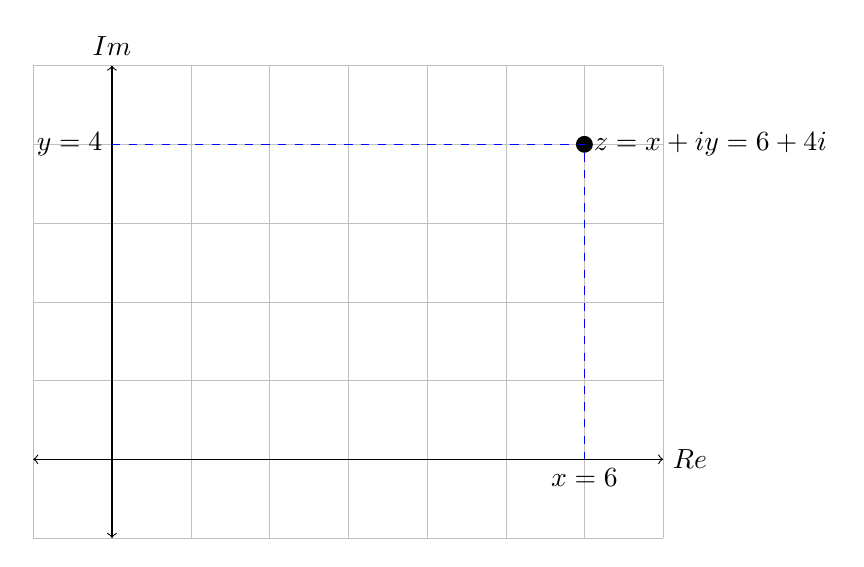
\begin{tikzpicture}
        \draw [ultra thin, lightgray] (-1,-1) grid (7,5);
        \draw [<->] (-1, 0) -- (7, 0) node[right] {$Re$};
        \draw [<->] (0, -1) -- (0, 5) node[above] {$Im$};
        \draw [black, fill = black] (6,4) circle [radius = 1 mm]
            node[black, right] {$ z = x + iy = 6 + 4i $};
        \draw [blue, dashed] (0,4) node[black, left] {$ y = 4 $}
            -| (6,0) node[black, below] {$ x = 6 $};
    \end{tikzpicture}
    \\ \\

    Misal $ z_1 = ( x_1 , y_1 )  $ dan $ z_2 = ( x_2 , y_2 ) $, maka berlaku:

    \begin{align}
            z_1 + z_2   & = ( x_1 \;,\; y_1 ) + ( x_2 \;,\; y_2 )
            \nonumber\\
            & = ( x_1 + x_2 \;,\; y_1 + y_2 )
            \\\nonumber\\
            z_1 \cdot z_2   & = ( x_1 \;,\; y_1 ) \cdot ( x_2 \;,\; y_2 )
                            \nonumber\\
                            & = ( x_1 x_2 - y_1 y_2 \;,\; x_1 y_2 + x_2 y_1 )
                            \\\nonumber\\
            a \cdot z_1 & = a \cdot ( x_1 \;,\; y_1 )
                        \nonumber\\
                        & = ( ax_1 \;,\; ay_1 )
    \end{align}
    \\ \\

    \newpage
    \begin{center}
        \textbf{Modulus Bilangan Kompleks}
    \end{center}
    \leavevmode\\

    Modulus atau nilai absolut bilangan kompleks $ z = x + iy $, didefinisikan sebagai bilangan real tidak negatif yang merupakan panjang vektor posisi dari $z$ (jarak antara $z$ dengan pusat sumbu).
    \\ \\

    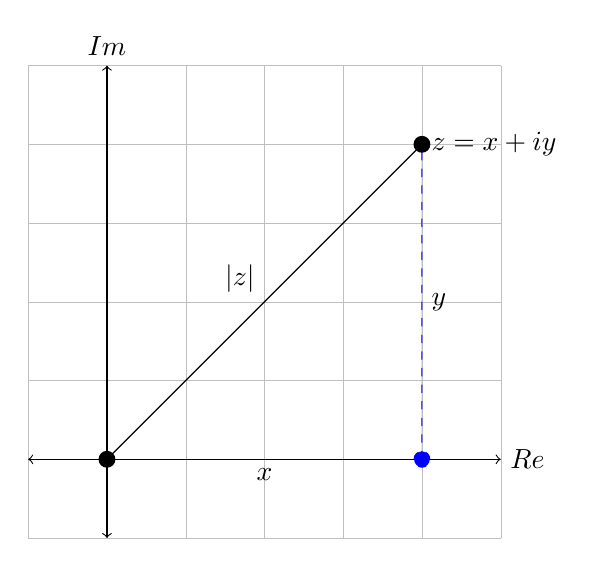
\begin{tikzpicture}
        \draw [ultra thin, lightgray] (-1,-1) grid (5,5);
        \draw [<->] (-1, 0) -- (5, 0) node[right] {$Re$};
        \draw [<->] (0, -1) -- (0, 5) node[above] {$Im$};
        \draw [black, fill = black] (4,4) circle [radius = 1 mm] 
            node[black, right] {$ z = x + iy $};
        \draw [black, fill = black] (0,0) circle [radius = 1 mm] -- (4,4);
        \draw [dashed, blue, fill = blue] (4,0) circle [radius = 1 mm] -- (4,4);
        \draw (2,2) node[above, anchor=south east, black] {$|z|$};
        \draw (4,2) node[right, black] {$y$};
        \draw (2,0) node[below, black] {$x$};
    \end{tikzpicture}
    \\ \\

    \begin{align}
        |z|         &= \sqrt{x^2+y^2}
        \\\nonumber\\
        |z_1 - z_2| &= \sqrt{(x_1-x_2)^2 + (y_1-y_2)^2}
    \end{align}
    \\ \\

    Sifat Modulus
    \begin{align}
        \bigg | \frac{z_1}{z_2} \bigg | &= \frac{|z_1|}{|z_2|}
        \\\nonumber\\
        |z_1 z_2|                       &= |z_1| \cdot |z_2|
    \end{align}
    \\ \\

    \newpage
    \begin{center}
        \textbf{Sekawan/\textit{Konjugate} Bilangan Kompleks}
    \end{center}
    \leavevmode\\

    Misalkan $ z = x + iy $, sekawan dari $z$ (notasi = $\overline{z}$) adalah pencerminan dari $z$ terhadap sumbu real ($R$).
    \\ \\ 

    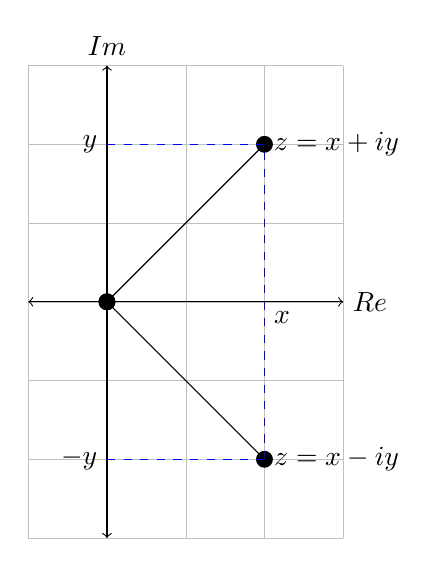
\begin{tikzpicture}
        \draw [ultra thin, lightgray] (-1,-3) grid (3,3);
        \draw [<->] (-1, 0) -- (3, 0) node[right] {$Re$};
        \draw [<->] (0, -3) -- (0, 3) node[above] {$Im$};
        \draw [black, fill = black] (2,2) circle [radius = 1 mm] 
            node[black, right] {$ z = x + iy $};
        \draw [black, fill = black] (2,-2) circle [radius = 1 mm] 
            node[black, right] {$ z = x - iy $};
        \draw [black, fill = black] (0,0) circle [radius = 1 mm] -- (2,2);
        \draw [black, fill = black] (0,0) circle [radius = 1 mm] -- (2,-2);
        \draw [dashed, blue] (2,-2) -- (2,2);
        \draw [dashed, blue] (0,2) node[left, black] {$y$} -- (2,2);
        \draw [dashed, blue] (0,-2) node[left, black] {$-y$} -- (2,-2);
        \draw (2,0) node[below right, black] {$x$};
    \end{tikzpicture}
    \\ \\ \\ \\

    Sifat Sekawan/\textit{Konjugate}:
    \begin{itemize}
        \item $\overline{z_1 + z_2} = \overline{z_1} + \overline{z_2}$
        \item $\overline{z_1 z_2} = \overline{z_1} \cdot \overline{z_2}$
        \item $|z| = \overline{z}$
        \item $\overline{zz} = |z|^2$
        \item $Re(z) = \dfrac{z+z}{2}$\\ \\
            $Im(z) = \dfrac{z-z}{2i}$
    \end{itemize}

    \newpage
    \begin{center}
        \textbf{Representasi Polar}
    \end{center}
    \leavevmode\\

    Misalkan $r$ dan adalah koordinat polar dari titik $(x, y)$ bilangan kompleks bukan nol $z = x + iy$. Karena $x = r cos \theta $ dan $y = r sin \theta$, maka bilangan Kompleks $z$ dapat
    ditulis dalam bentuk polar:

    \begin{align}
        z = r(cos \theta + i sin \theta)\\\nonumber
    \end{align}

    dengan,
    \begin{itemize}
        \item r adalah modulus dari $z$:\\
            $ r = |z| = \sqrt{x^2+y^2} $
        \item $\theta$ adalah argumen dari $z$:\\
            $ \theta = tan^{-1} \bigg(\dfrac{y}{x}\bigg) $
    \end{itemize}

    \leavevmode
    \\ \\ \\ \\

    \begin{center}
        \textbf{Representasi Euler}
    \end{center}
    \leavevmode\\

    Notasi matematis formal adalah bentuk Euler:
    \begin{align}
        z = re^{i\theta}\\\nonumber
    \end{align}

    Identitas Euler:
    \begin{align}
        e^{i\theta} = cos\theta + i sin\theta \\\nonumber
    \end{align}

    \newpage
    \begin{center}
        \textbf{Perkalian dan Pangkat Bentuk Exponen}
    \end{center}
    \begin{align}
        e^{i\theta_1} e^{i\theta_2} &= (cos\theta_1 + i sin\theta_1)(cos\theta_2 + i sin\theta_2)
                                    \nonumber\\
                                    &=(cos\theta_1 cos\theta_2 - sin\theta_1 sin\theta_2) + i(sin\theta_1cos\theta_2 + cos\theta_1 sin\theta_2)
                                    \nonumber\\
                                    &= cos(\theta_1 + \theta_2) + i\;sin(cos(\theta_1 + \theta_2))
                                    \nonumber\\
                                    &= e^{i(\theta_1 + \theta_2)}
    \end{align}
    
    Maka, jika $z_1 = r_1e^{i\theta_1}$ dan $z_2 = r_2e^{i\theta_2}$, produk $z_1z_2$ memiliki bentuk eksponensial:
    \begin{align}
        z_1z_2  &= r_1e^{i\theta_1} r_2e^{i\theta_2}
                \nonumber\\
                &= r_1r_2e^{i\theta_1}e^{i\theta_2}
                \nonumber\\
                &= (r_1r_2)e^{i(\theta_1\theta_2)}
    \end{align}
    \begin{align}
        \dfrac{z_1}{z_2}    &= \dfrac{r_1e^{i\theta_1}}{r_2e^{i\theta_2}}
                            \nonumber\\
                            &= \dfrac{r_1}{r_2} \cdot \dfrac{r_1e^{i\theta_1}}{r_2e^{i\theta_2}} \cdot \dfrac{e^{-i\theta_2}}{e^{-i\theta_2}}
                            \nonumber\\
                            &= \dfrac{r_1}{r_2} \cdot \dfrac{e^{i(\theta_1-\theta_2)}}{e^{i0}}
                            \nonumber\\
                            &= \dfrac{r_1}{r_2} e^{i(\theta_1-\theta_2)}
    \end{align}
    \begin{align}
        z^{-1}  &= \dfrac{1}{z}
                \nonumber\\
                &= \dfrac{1e^{i0}}{re^{i\theta}}
                \nonumber\\
                &= \dfrac{1}{r} e^{i(0-\theta)}
                \nonumber\\
                &= \dfrac{1}{r} e^{-i\theta}
    \end{align}
    \begin{align}
        z^n &= r^n e^{in\theta}
    \end{align}

    \newpage
    \begin{center}
        \textbf{Fungsi Kompleks}
    \end{center}
    \leavevmode\\

    Fungsi kompleks $f(z)$ menyatakan pemetaan dari bidang kompleks asal $z$ (domain) ke bidang kompleks hasil $w$ (range) dengan suatu pola yang diatur oleh $f(z)$.
    \\

    Contoh (titik ke titik):
    \begin{align}
        f(z)    &= 2z + 1
                \nonumber\\
                &= 2(x+iy) + 1
                \nonumber\\
                &= 2x + 2iy + 1
                \nonumber\\
                &= (2x + 1) + 2iy
                \\\nonumber\\
        Re(z)   &= u(x,y) = 2x + 1
                \nonumber\\
        Im(z)   &= v(x,y) = 2y
                \nonumber
    \end{align}
    
    Contoh (lintasan ke lintasan):
    \begin{align}
        f(z)    &= \overline{z}
                \nonumber\\
                &= x - iy
                \\\nonumber\\
        Re(z)   &= u(x,y) = x
                \nonumber\\
        Im(z)   &= v(x,y) = -y
                \nonumber
    \end{align}

    Contoh (daerah ke daerah):
    \begin{align}
        f(z)    &= z + 1
                \nonumber\\
        D : |z| &<1
                \nonumber\\
        f(z)    &= z + 1
                \nonumber\\
        w       &= z + 1
                \nonumber\\
        z       &= w - 1
                \nonumber\\
        |w-1|   &< 1
                \\\nonumber
    \end{align}
    \\

    \begin{center}
        \textbf{Titik Singular}
    \end{center}
    \leavevmode\\

    Titik dimana $f(z)$ gagal dipetakan ke titik lain. Contoh pada fungsi \\ $f(z) = \dfrac{1}{z+1}$ gagal dipetakan pada titik asal $z=1$ karena $\dfrac{0}{0}$ tidak terdefinisi.

    \newpage
    \begin{center}
        \textbf{Limit Fungsi Kompleks}
    \end{center}
    \leavevmode\\

    Konsep limit pada fungsi kompleks $f(z)$ diperluas dari limit pada fungsi real $f(x)$ sebagai:
    Pada fungsi kompleks $f(z)$, $\lim_{z \to z_0} f(z)$ bernilai $L$ atau
    \begin{align}
        \lim_{z \to z_0} f(z) = L
    \end{align}
    jika terdapat $\epsilon  > 0$ dan $\delta  > 0$ sedemikian sehingga jika ada $\epsilon$ yang memenuhi $|f(z) - L| \leq \epsilon$ , maka terilustrasi:
    \begin{itemize}
        \item $|z - z+0| \leq \delta$ adalah disk dengan pusat di $z_0$ dan jari-jari $\delta$
        \item $|f(z) - L| \leq \epsilon$ adalah disk dengan pusat di $L$ dan jari-jari $\epsilon$
    \end{itemize}
    \leavevmode\\ \\

    \begin{center}
        \textbf{Turunan Fungsi Kompleks}
    \end{center}
    \leavevmode\\

    Aturan penurunan pada fungsi riil berlaku pada fungsi kompleks. Jika $f(z)$ dan $g(z)$ adalah dua fungsi kompleks, maka:
    \begin{itemize}
        \item penjumlahan
        \begin{align}
            \frac{d}{dz}(f(z)+g(z)) &= f'(z) + g'(z)
        \end{align}
        \item perkalian skalar
        \begin{align}
            \frac{d}{dz}(kf(z)) &= kf'(z)
        \end{align}
        \item aturan rantai
        \begin{align}
            \frac{d}{dz}(f(g(z))) &= f'(g(z)) g'(z)
        \end{align}
        \item aturan perkalian
        \begin{align}
            \frac{d}{dz}[f(z)g(z)] &= f'(z)g(z) + g'(z)f(z)
        \end{align}
        \item aturan pembagian
        \begin{align}
            \frac{d}{dz}\frac{f(z)}{g(z)} &= \frac{f'(z)g(z) - g'(z)f(z)}{g^2(z)}
        \end{align}
    \end{itemize}
\end{document}